\spread{Reading the words on either side of an answer}
\noindent A question about what a person decided to become calls for an occupation. A location in the same passage can be equally easy to copy. We asked whether a model could learn to distinguish the two from the order of the pictured context.
\platehere{Figure_176_reading_the_evidence_in_order}{Finding the right phrase and writing the right sentence can come apart}{The rows reproduce the actual selected strips and freely emitted replies. Panel a shows the first English gain in exact evidence over the earlier reader within the display budget. The directed reader selects the occupation, but the writer introduces it twice. Panel b shows the corresponding first Chinese loss. The earlier reader gives the accepted short answer. The directed reader includes that answer within a longer passage about several possible outcomes. Both examples were selected by an exact image criterion.}
\begin{multicols}{2}
\section*{An order-sensitive correction}
For each possible endpoint $i$, we pool the pictured context on its left and right over four widths (4, 16, 64 and 256 cells). Both readers see the local page state, the question and $R_i+L_i$. One also sees $R_i-L_i$, the other $|R_i-L_i|$. Both train 25,026 parameters. They score all legal spans before the same frozen ranker selects from the best 32. The frozen sentence writer receives the pictured question and the selected strip. No external language model supplies its answer.
\section*{A prediction that can be checked}
A deterministic rule with an exchange-invariant representation makes the same prediction on a pair of exchanged inputs. It therefore cannot recover two different labels on that pair. Lean verifies this implication and the reversal of a signed margin. The inherited reader already sees local order. We therefore exchanged only the two pools in the added correction. On 192 new English questions, exact evidence fell from 43 to 21 for the signed reader. All 192 choices of the unsigned reader stayed fixed. This intervention identifies a mechanism that the trained model actually used.
\section*{What the Chinese image contains}
Of 192 Chinese evidence strips, 14 matched a human answer, 57 strictly contained one and 16 were a proper part of one. The other 105 had neither containment relation. The earlier reader produced 34 overlong strips. A longer strip can preserve the requested fact, as in panel b, or obscure it among competing claims. Giving the unchanged writer the first visible accepted span raised exact replies from 13 to 181 on 189 Chinese questions. On the 192 English questions, stopped replies containing the fact rose from 47 to 141, yet none matched the short reference exactly. Human evidence was supplied only in this intervention.
\end{multicols}
\newpage
\spread{How far does better evidence carry the answer?}
\noindent The two readers saw the same 39,057 English and Chinese training questions four times. We tested them on 96 previously reserved pages in each of three cohorts, asking two different questions per page.
\platehere{Figure_177_learning_to_locate_evidence}{Trading training loss for held evidence and complete answers}{\textbf{a}, The count requires exact agreement between the selected pixels and an accepted answer. English and Chinese use monolingual MLQA test passages. The third cohort uses English DROP passages with a single distinct nonempty annotation string. An optical overlap audit found no complete question or page in the two supervised parent pools. Six questions shared a sampled 64-cell passage fragment with training. \textbf{b}, Mean training negative log likelihood of the annotated span locations over each complete epoch, measured before reranking. The writer remained fixed.}
\begin{multicols}{2}
\section*{Three independent reading outcomes}
English evidence improved from 30 to 43 of 192 against the earlier reader and from 37 to 43 against the unsigned one. The latter difference was 3.1 percentage points (paired page-bootstrap 95\% interval, 0.5--6.3). Correct evidence in Chinese remained at 14, and on DROP it rose from six to nine. Only 107 of the 192 DROP questions had a reference string visible in the supplied passage. Among the signed reader's best 32 candidates, an accepted strip occurred for 131 English and 77 Chinese questions. The final selection missed 88 and 63 of these, respectively. The checked finite-list bound partitions the remaining errors into 61 and 115 questions without an accepted candidate. In English, 47 stopped answers contained the human fact, but none exactly matched a short reference. In Chinese 13 complete answers matched.
\section*{Reading for meaning}
On the first eight reserved pages in each cohort, we compared the complete replies with those of a quantized Qwen3-VL 8B reader given the same pictured content. A separate quantized Qwen3 8B judge read anonymized candidates in two opposite orders. It credited the signed model on 2/16 English MLQA, 6/16 Chinese MLQA and 0/16 DROP questions; Qwen3-VL earned 10, 15 and eight. Human reference controls earned 47/48 and sibling-question foils were rejected twice on 47/48. This small model-judged comparison measures task-specific answer adequacy.
\section*{Cost and remaining failures}
The directed update took 44.3 seconds and 7.28 kJ on one RTX 4090 D. For the 48-question comparison, the compact pipeline used 0.31 kJ of device energy and Qwen3-VL used 14.4 kJ. The models reached different levels of accuracy. These figures exclude previous training and host energy. Neither new reader returned an exact held long-form reply on 128 prompts or identified the requested historical specimen in the 260 bilingual period tests. Evidence selection transfers further than independent composition in this experiment.
\end{multicols}
\begin{center}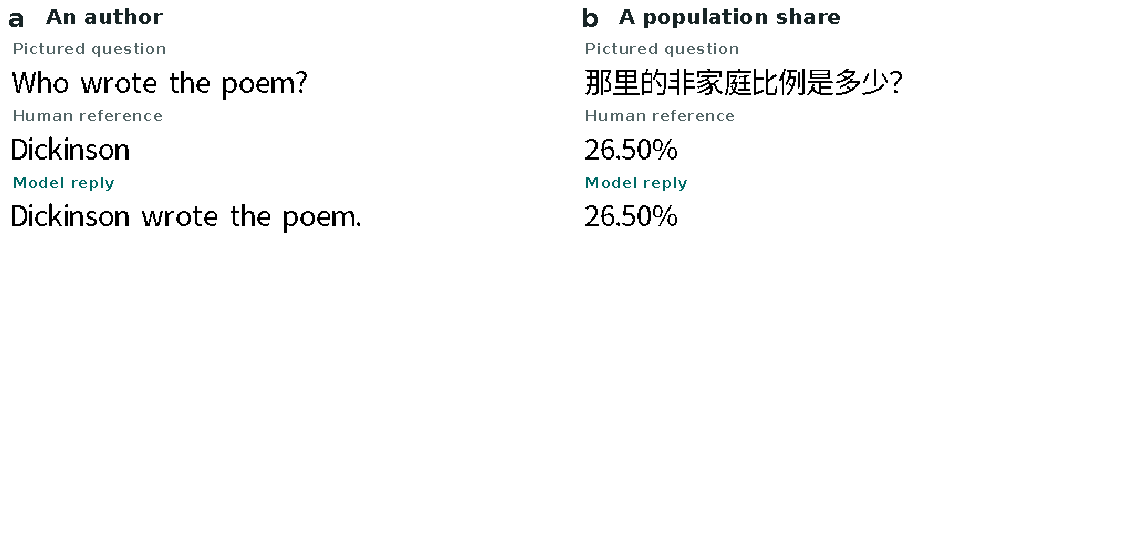
\includegraphics[width=.9\linewidth,trim=0 150bp 0 0,clip]{../figures/Figure_178_two_complete_visual_replies.pdf}\end{center}
\noindent{\small\textbf{Two credited replies.} First stopped reply credited in both judgment orders in each MLQA cohort. The English answer supplies a verb and object around the selected name. The Chinese answer gives the requested percentage. The response rows are the emitted images.}
\smallskip\noindent{\small\sffamily\textbf{Corpora.} Lewis et al., \href{https://aclanthology.org/2020.acl-main.653/}{MLQA} (2020); Dua et al., \href{https://aclanthology.org/N19-1246/}{DROP} (2019).}
\newpage
